\chapter{\textbf{Literature review}}  \label{chapter:lit}

According to \cite{chowdhury2003} ``Natural Language Processing (NLP) is an area of research and application that explores how computers can be used to understand and manipulate natural language text or speech to do useful things''. In order to build the right tools and techniques to enable computer systems to comprehend and manipulate natural languages to carry out specified tasks, researchers in natural language processing seek to learn about how people interpret and use language.\\

Working with quantitative and qualitative data simultaneously is one of the benefits of using documents, texts, and minutes \cite[p. 1]{bholat2015text}. Even while these types of studies have a wide range of applications, they have only recently been employed in economics despite the fact that working with both types of data makes it possible to conduct research and draw statistical inferences that are not achievable with simply structured data. In this way, it would be possible to have a better understanding of what happens in the economic scenario behind models that we work with NLP -- understanding feelings and emotions of economic agents has always been a goal of science, whether for a better understanding of its uses or even in terms of behavior of the consumer.\\

\section{Measuring News Sentiment}

In a recent study, \cite{shapiro2020measuring} presents new evidence that incorporate NLP techniques into economic science. According to the authors, it was possible to obtain a sentiment index that matched the Michigan Consumer Sentiment Index (MCSI)\footnote{\url{http://www.sca.isr.umich.edu/}}, from economic articles and assessed financials. In terms of methodology, it would then be possible to obtain an index of consumer sentiment through selected journals and textual sentiment analysis techniques.\\

The authors start from the lexicons GI \cite[]{heston2017news}, LM \cite[]{loughran2011liability}, and HL \cite[]{hu2004mining} and test their predictive capacity against human ratings and from there, classify the models of according to goodness-of-fit measures. The LM and HL lexicons obtained similar and superior results compared to GI. Once this is done, the authors also consider the union of the three lexicons, so that human ratings are now tested against ``GI + LM + HL lexicon'' \cite[p. 13]{shapiro2020measuring}. The authors still use VADER \cite[]{hutto2014vader} due to its predictive ability and its ``negation rule'' \cite[]{potts2010negativity}, unfortunately, the authors point out ``Vader is designed for the social-media domain, not the
economics/ finance domain'' \cite[p. 14]{shapiro2020measuring}.\\

For a solution around the predictability of lexicons, the authors decide to create their own lexicon, through their composition (and the inclusion of VADER's negation terms). Having done that, the article then proposes the creation of a sentiment index based on this lexicon, so that a monthly sentiment index was estimated from fixed effects ($\hat{f}_{t(a)}$ ), given the regression:

\begin{align*}
    s_a = f_{p(a), j(a)} + \varepsilon_a \quad ,
\end{align*}
where $s_a$ is the net positivity score for article $a$ and $f_{t(a)}$ is a sample-month ($t$) fixed effect. Newspapers are indexed by $j$ and article type -- either editorial or regular article -- is indexed by $p$ \cite[p. 20]{shapiro2020measuring}. So, $f_{p(a), j(a)}$ is the fixed effect of newspaper*type: this ensures that the index is independent of changes over time, relative to its composition of newspapers and editorials, when compared to regular articles. This might be significant, as the tone of articles varies greatly between newspapers and between editorials and ordinary articles within a newspaper.\\

Two main studies were proposed: first, it would be analyzed whether the sentiment index elaborated by the authors would be a good predictor variable for real economic variables. For this exercise, the authors used three variable selection models as a methodological approach: a LASSO, an Adaptive LASSO, and a Group LASSO. Variable selection models showed that the sentiment index is significant in the predictor aspect, even when compared to the Michigan Consumer Sentiment Index, the LASSO Group points out the authors' index (based on sentiment techniques) as superior in some models ` `Specifically, at least one of the versions of LASSO prefers the measure of news sentiment in forecasts of employment, output (IP), inflation, real rate (FFR) and S\&P 500'' \cite[p. 26]{shapiro2020measurement}. The economic variables used for this study were: employment, output, inflation, real rate, consumption, S\&P 500, MCSI and Conference Board Consumer Confidence Index, in addition to the authors' sentiment index.\\
In a second exercise carried out by the authors, it was analyzed how economic activity would react to a positive shock in the sentiment index. Unlike the conventional method (from an autoregressive vector), the impulse response functions were obtained through local projections \cite{jorda2005estimation} (similar to VAR, but with a less restrictive approach). The results obtained demonstrate that a positive shock in the sentiment index would lead to a slight increase in consumption, in the economy's output, in the real interest rate and in the price level. In addition to these results, impulse responses were also estimated for the Michigan Consumer Sentiment Index and the Conference Board's Consumer Confidence index (CBCI). When analyzing the responses of economic activity to the MCSI, the economic variables (with the exception of the interest rate that responds positively) were not statistically significant. When analyzing the responses of the economic variables to a CBCI choue, the results are similar to the results obtained with the authors' sentiment index -- the responses of the economic variables are statistically significant and point to a slight increase.\\

From economic articles, then, it is possible to analyze and better understand the economic situation. The extraction of a sentiment index through NLP techniques also saves the time and funds needed to obtain an index of this content. With the passage of time, the NLP techniques will evolve, allowing, thus, an improvement in the computational field and in the part of sentiment analysis applied to the economy.\\

\section{Taking the fed at its word: A New Approach to Estimating Central Bank Objectives Using Text Analysis}

In another article, \cite{shapiro2021taking} analyzes Federal Reserve deliberations from NLP techniques to estimate central bank preferences. In other words, it would be possible to estimate the objective function of some generic central bank from its speeches or internal meetings.\\

Based on the estimation of the central bank's loss function, the results showed that the inflation target for the analyzed period (2000-2011) was approximately 1.5\%. With this result, it is possible to perceive that, as everything indicates, the value of the inflation target would be, therefore, significantly below what the surveys of inflation expectations indicated in the period -- for the long term. However, it has been documented \cite[p.32]{shapiro2021taking} that the position of certain members of the Federal Open Market Committee\footnote{Where the speeches come from.} have sometimes stated that an inflation target of 1.5\% seemed consensus at least until 2009 -- after this period, the inflation target value would be 2.0\%.\\

The article also finds that the ``negativity'' of the FOMC is most affected by economic growth and financial conditions. This statement is supported by \cite{walsh2003speed}, which addresses how central banks end up focusing more on economic growth and \cite{coibion2011monetary} which raises this hypothesis based on empirical estimations of the Taylor rule. In a previous work, \cite{thornton2011does} has already pointed out that the FOMC ends up focusing more on the issue of ```growth in output', and not sustainable employment, the unemployment rate, or any concept of slack, as part of their policy directive from 1979 through 2008'' \cite[p.34]{shapiro2021taking}. A question also raised by the article was how financial variables would behave in the face of FOMC speeches. \cite{bernanke2001should} points out that monetary policy should not, for example, respond to a change in asset prices. Having an opinion that supports this study, former Fed Vice President Don Kohn says that the Fed does not respond to asset prices \cite{kohn2006monetary, kohn2009monetary}.\\

On the other hand, a study by \cite{peek2015should} presents financial variables as good predictors of the Fed's interest rate, when these are incorporated into a Taylor rule that takes into account financial instabilities. Finally, \cite{cieslak2021economics} points out that both a stock market crash and a real negative stock market return affect FOMC discourses, and thus become predictive variables of the Fed's interest rate.\\

\section{Information, Animal Spirits, and the Meaning of Innovations in Consumer Confidence}

In another article, to better investigate consumer behavior and sentiment, \cite{barsky2012information} developed two fundamental strategies: the estimation of a New Keynesian Dynamic Stochastic General Equilibrium DSGE, and the estimation of several VAR models. Through the answer of a question, ``Turning to economic conditions in the country as a whole, do you expect that over the next five years we will have mostly good times, or periods of widespread unemployment and depression, or what?'' \cite[p.1347]{barsky2012information}, the authors created a variable (E5Y) so that this is the percentage of favorable answers to the question minus the percentage of negative answers to the question plus 100. The authors did the same, then, to a horizon of 12 months ahead, and called the variable E12M, in order to better understand how expectations would vary in different future timeframes. Also, they create the expected personal financial (PFE) variable, according to the answer ``Now looking ahead -- do you think that a year from now you (and your family living there) will be better off financially, worse off, or just about the same as now?'' \cite[p.1371]{barsky2012information} and finally create a consumer expectation index (ICE) according to the equation:

\begin{align} \label{eq:ice}
    ICE = \frac{PFE + E12M + E5Y}{4.1134} + 2.0
\end{align}

another index, the consumer sentiment index (ICS) is developed from a variation of the equation (\ref{eq:ice}):

\begin{align} \label{eq:ics}
    ICE = \frac{PFE + E12M + E5Y + DUR + PFP}{6.7558}
\end{align}

where in the equation (\ref{eq:ics}) DUR represents ``wheater or not it is currently a good time to buy `large household items''' \cite[p.1372]{barsky2012information} and PFP is identical `` to PFE, except that PFP respondents to compare their current financial situation relative to one year ago''\cite[p.1372]{barsky2012information}.\\

Based on this interest in a possible sentiment index, the authors estimated VAR models in order to understand how this index would behave if modeled against variables of economic activity. The authors demonstrate from impulse response functions that economic variables such as consumption would have, given a positive shock on the sentiment index, a temporary positive change. The same happens when analyzing the output of the economy.\\

The authors go further and implement a new Keynesian DSGE model incorporating into the model an ``animal spirit'' effect interpreted as ``noise innovations in the signal about productivity growth''\cite[p.1353]{barsky2012information} and trust, represented by E5Y. Assuming that agents observe the technology level from period to period, a noisy signal of the growth rate can be observed:
\begin{align*}
     s_t = g_t + \varepsilon_{s,t}
\end{align*}
where $g$ is an AR(1) stationary process of growth and the shock $\varepsilon_{s,t}$ is interpreted as the animal spirit shock. E5Y in turn is modeled according to the autoregressive process:
\begin{align*}
     E5Y_t = (1 - \rho_e) + \rho_e E5Y_{t-1} + u_t
\end{align*}
where $u_t$ represents the innovation in confidence\footnote{$u_t$ is also modeled as an autoregressive process of order 1. For further explanation, see \cite[p.1354]{barsky2012information}}.\\

The objective of the DSGE estimation was to compare the results of the impulse responses of an anial spirit shock with the results obtained in the VAR models. This ends up having repercussions on another question: ``why are confidence innovations prognostic of future movements in economic activity''\cite[1356]{barsky2012information}? The estimation results corroborate previous studies \cite{rotemberg1997optimization, christiano2005nominal} on the topic.\\

The theoretical impulse responses obtained from the DSGE present interesting results in relation to the shock in the animal spirit variable. First, given a shock in this variable, the response of the economy's output would be a decrease with an ever growing in the first post-shock periods, with a gradual return to its steady state in about 10 periods. The inflation response to a shock in the animal spirits variable would be a decrease in the first period with a gradual return to its steady state around 10 periods; and finally, the interest rate would undergo a slight positive variation in the first 3 periods, with a gradual return to its steady state in about 7 periods. The DSGE also analyzes the response of the consumer confidence index to a positive shock in animal spirit: this variable would respond positively to a positive shock in animal spirit, unlike the other variables, the temporary effect of consumer confidence would be present until the return from this variable to its steady state, in just over 20 periods.\\

The DSGE model assumes, though, that the animal spirit variable would affect the economy from its technology level, thus affecting the product. While the impact on the product is only slightly significant, this may be due to the calibration of the model. The authors calibrated the DSGE so that it followed a certain level of price rigidity: ``in other words, prices are almost perfectly rigid and the central bank does not adjust interest rates to output fluctuation''\cite[p.1365]{ barsky2012information}. The results obtained through the DSGE were similar to the results obtained in \cite{l2009news}.\\

\section{Sentiments}

In another article, \cite{angeletos2013sentiments} investigates, also through a DSGE model, how the issue of ``market sentiments'' and ``animal spirit'' affects the equilibrium of the economy. The model also investigates what would be the effect of limited communication within a neoclassical economy, where commerce is random and decentralized. It is shown, then, that the business cycle responds to exogenous shocks of sentiment through technology, and the propagation of these shocks depends directly on the communication condition of the economy.\\

The model developed by the authors considers the economy divided into several ``islands'' \cite{lucas1972expectations}, so that it is heterogeneous in terms of exchange opportunities, productivity factor and information. The model incorporates the sentiment shock as a random shock into the factor of productivity equation, so that:
\begin{align} \label{ep:dsgesentiment}
     x_{it} = x_{jt} + \xi_t + i_{it}
\end{align}
where $\xi_t$ would represent the sentiment variable in the productivity factor equation (\ref{ep:dsgesentiment}). This variable $\xi$ is affected when, for example, a firm makes an important production or employment decision and does not have the option of warning or communicating to consumers who it will find or exchange goods or even whose decision will be determine the profitability of the firm \cite[p.741]{angeletos2013sentiments}.\\

The results found by the authors indicated that the exogenous shocks of technology were propitiated, in the authors' view, by the shocks of ``feelings''. ``These shocks impact the information that is available to each island, without, however, affecting the latter's beliefs either about the aggregate fundamentals or about the idiosyncratic fundamentals of its trading partner'' \cite[p.742]{angeletos2013sentiments}. According to the authors, these clashes can also be called ``higher-order beliefs''. The specific type of higher-order uncertainty is then eliminated by requiring the aggregate fundamentals to be defined and well known, as previously pointed out by \cite{morris2002social, woodford2001imperfect}. ``Nevertheless, by introducing trading frictions and imperfect communication, we open the door to higher-order uncertainty at the micro level: when two islands are matched together, they are uncertain, not only about each other's productivity, but also about each other's beliefs of their productivity, each other's beliefs of their beliefs of their productivity, and so on. The fluctuations
we document reflect correlated variation in this kind of higher-order beliefs'' \cite[p.742]{angeletos2013sentiments}.\\

The authors thus tried to explain the origins of exogenous shocks in economic fluctuations through sentiment shocks. The question that still remains open is whether these shocks could be shifts in preference and shifts in technology or even waves of pessimism and optimism in the economy. Despite using an approach that does not use NLP techniques, the search for measuring sentiments in the economy seems to reveal the importance of this abstract variable for a better understanding of the behavior of economic agents.\\

\section{Macroeconomic Expectations: News Sentiment Analysis}

Trying to extract sentiments from newspaper news and scientific articles to identify whether they affect macroeconomic variables, \cite{ostapenko2020macroeconomic} obtains a sentiment index from ``topic models'' and a representation of the documents grouped by clusters. Each type of article ended up impacting a specific area or sector of economic activity: ``Articles about the
economy are found to be the most important for their expectations for interest rates, articles about loans matter most for in action expectations, and articles about housing are the most relevant for unemployment expectations'' \cite[p.2]{ostapenko2020macroeconomic}. To understand how the sentiment index obtained relates to the real activity of the economy, the author chose to estimate a VAR: ``The VARs for real economic activity also include the logarithm of industrial production, the logarithm of real personal consumption expenditures, the logarithm of the PCE price
index, the federal funds rate, and the consumer sentiment index. The VARs for monetary policy use the logarithm of industrial production, the logarithm of the consumer price index, the one-year constant-maturity Treasury yield as a monetary policy indicator, and the excess bond premium as an indicator of financial conditions'' \cite [p.2]{ostapenko2020macroeconomic}.\\

The results found by the author indicate that the output of the economy suffered a variation of 20\% for a long-term horizon given a shock in the sentiment index. This clash of sentiments is also related to an increase in consumption, inflation and interest rates, albeit as a temporary change. Furthermore, the study pointed out that in terms of magnitude, a shock to the sentiments variable is more important, in long-term terms, than a shock to consumer sentiments. ``The study nds that a soft news shock accounts for about 20\% of the forecast error variance of output at long horizons. decomposing the main component by soft news shocks to separate topics accounts for about 7-27\% of the forecast error variance of output and about 5\% of the variance in consumption at long horizons in different models'' \cite[p.40]{ostapenko2020macroeconomic}. Compared with the other models estimated by the author, a shock in the sentiment index was similar to the results estimated by \cite{barsky2012information}, in terms of responses of economic variables to the shock. The results, when analyzing a shock to the Fed news, corroborate the previous literature \cite{jarocinski2020deconstructing, smith2015has} which points out that the Fed news may contain information that anticipates the outlook of the general economy -- the same happens when considering the shock of monetary policy news.\\


Text mining, sentiment analysis, and other tools enable the area of economics gradually gain a better understanding of what is going on and how structural or conjunctural events relate to social expressions. Understanding consumer behavior and how the media may affect or even alter an economic situation are both made possible by sentiment analysis. From a text or corpus, text mining makes it possible to extract both qualitative and quantitative information. NLP will eventually be employed more and more to improve our understanding of the world and economic science.\\


%
%\begin{figure}[!h]
%    \centering
%    \caption{Impulse response of a positive news sentiment shock on economic activity}
%    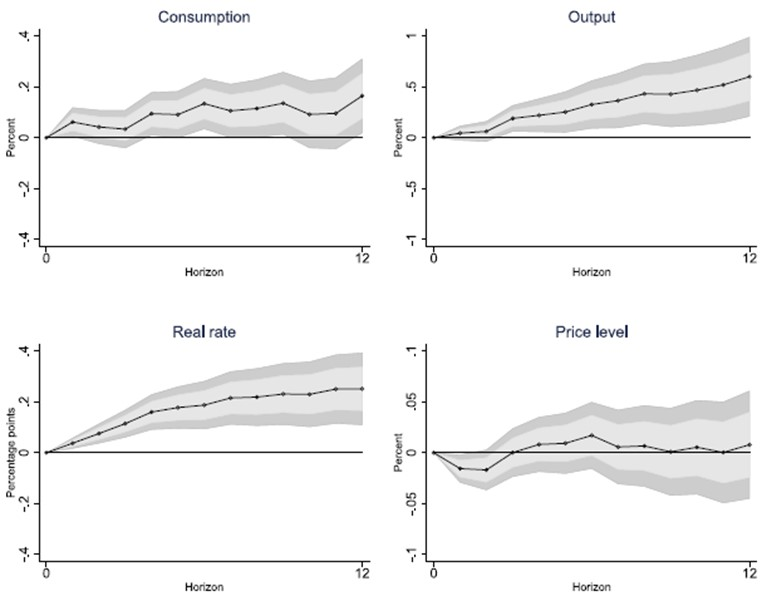
\includegraphics[width=.8\textwidth]{images/image1.jpg}
%    \caption*{Source: \cite[p.16]{shapiro2020measuring}}
%    \label{fig:my_label}
%\end{figure}














%In order to complement the literature of sentiment analysis in economics, \cite{ostapenko2020macroeconomic} contributed analysing “how the change of tone or topic in newspaper affects the macroeconomy”. The author transformed articles from newspaper (employing a topic model and vector representation of documents with clustering) into time series and based on this time series, evaluated the sentiment of each article. On occasion, the article demonstrated that given a new shock in the sentiment of the articles, it could mean an increase over the long run, in output and consumption – it also affects the inflation and interest rate, however transiently.\\

%Progressively, text mining, sentiment analysis and other techniques end up helping the field of economics to understand better what is happening and what is the relation of the conjunctural or structural scenarios with social expressions. Sentiment analysis helps to understand the consumption behaviour, or even how the media can influence or even chance an economic scenario. Text mining allows to extract qualitative and quantitative information from a text or a corpus. Sooner or later NLP will be increasingly used for a better understanding of the world or the field of economic science.\\


%In terms of descriptive analysis, or in terms of classifiers, the approach varies according to the chosen methodology, generally with greater emphasis on classification techniques such as support vector machine, k-means neighbours, or k-nearest neighbour (KNN) \citet{ostapenko2020macroeconomic}. Still, it is worth noting that approaches that assume NLP techniques such as tokenization (see section 3) are still little used, especially with regard to estimations: it is important to emphasize that not using techniques such as tokenization in estimations can create a lack of results in terms of contribution to economic science, given the fact that a better understanding of what happens in the economic scenario is possible and plausible based on a better understanding of how terms and expressions are related to economic cycles.\\



